\section{Background: Arweave and AO}

The Action substrate is built on AO, a revolutionary decentralized computing system that leverages Arweave's permanent data storage capabilities. To understand Action's architecture, it's essential to first grasp the foundational technologies it builds upon.

\subsection{AO: A Decentralized Computer}

Unlike traditional blockchains that operate as single-threaded systems with shared memory, AO functions as a decentralized computer that enables parallel execution of processes. This fundamental difference allows AO to support an unlimited number of concurrent processes without the scalability constraints typical of blockchain networks.

At its core, AO implements an actor-oriented paradigm where each process operates independently but can communicate through message passing\footnote{The actor-oriented paradigm in AO differs from traditional blockchain architectures by treating each process as an independent actor with its own state and behavior, rather than sharing a global state. This enables true parallel execution and eliminates the scalability bottlenecks common in traditional blockchain systems.}. This architecture creates a unified computing environment---a Single System Image---hosted across a distributed network of nodes. The result is a vast, scalable computer where users can interact with any process, fostering a highly collaborative ecosystem.

\subsection{Integration with Arweave}

AO uses Arweave as its persistent data layer, ensuring permanent availability of all process interactions and data. \cite{Williams2023} Rather than achieving consensus on computation results, AO ensures that logs of interactions are recorded and accessible on Arweave. This creates a `holographic' state system where the state may not have been computed by any participant yet but is guaranteed to always produce the same outputs when computed. \cite{Williams2024}

\subsection{Core Components}

AO's architecture consists of several key components that work together to enable decentralized computation, as shown in Figure \ref{fig:ao_architecture}:

\begin{figure}[ht]
\centering
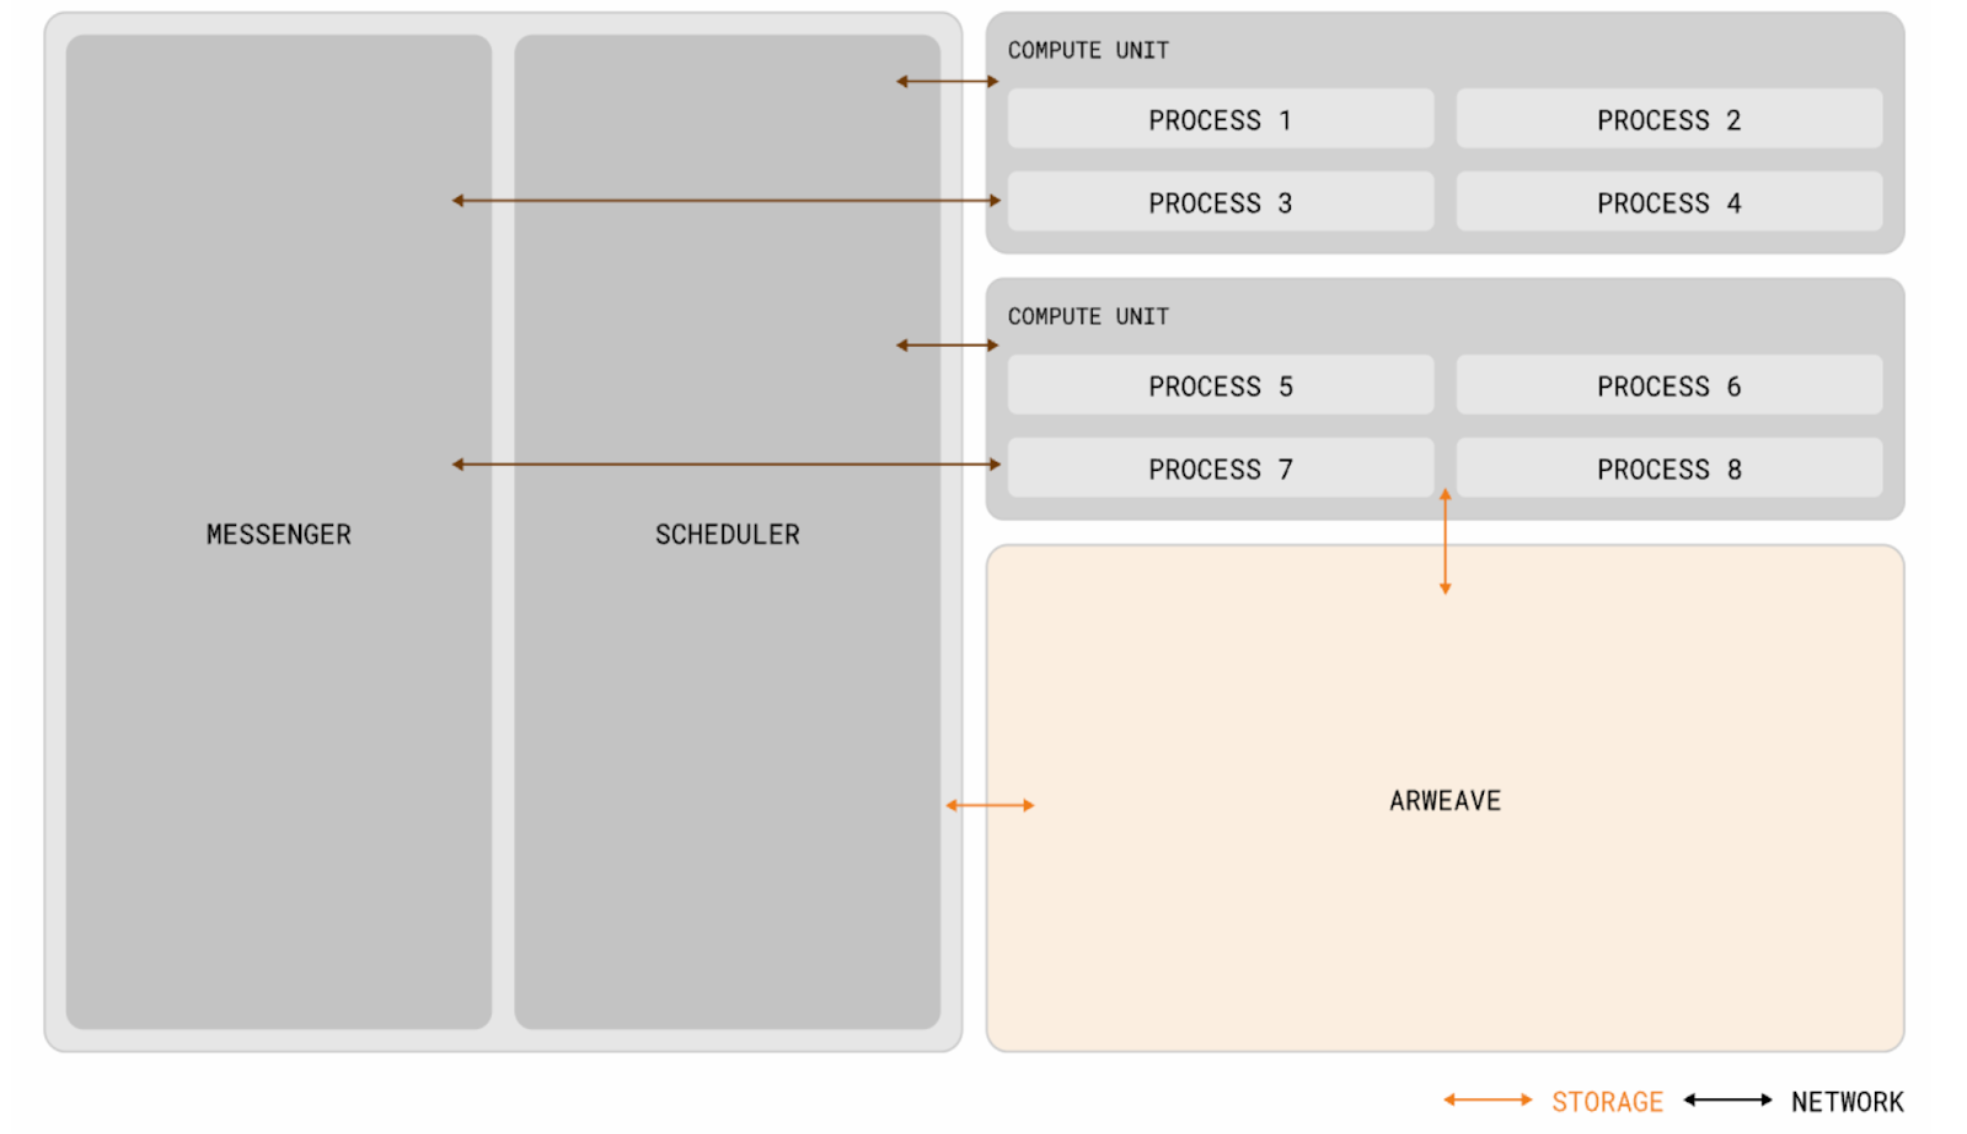
\includegraphics[width=\columnwidth]{images/image2.png}
\caption{The AO computer architecture takes a modular approach, splitting responsibilities into subnets where participants engage in peer-to-peer markets for service provision. \cite{Williams2024}}
\label{fig:ao_architecture}
\end{figure}

The fundamental building block is the \textbf{Process}, which represents the basic unit of computation in AO. Each process maintains a log of interacting messages stored on Arweave along with an initialization data item. Processes are highly configurable, defining their own computing environment including VM specifications, memory requirements, and necessary extensions.

\textbf{Messages} form the basis of all interactions within AO. Following the ANS-104 standard \cite{ANS104_2024}, messages are guaranteed to occur exactly once, with delivery confirmation ensured through Arweave's data persistence protocol\footnote{The ANS-104 standard ensures reliable message delivery through a combination of unique message IDs, cryptographic signatures, and Arweave's permanent storage. This guarantees that messages cannot be lost, duplicated, or tampered with, making it ideal for decentralized applications requiring strong consistency.}.

The system employs several specialized units to manage computation and communication. \textbf{Scheduler Units (SUs)} handle the critical task of assigning sequential slot numbers to messages sent to processes, ensuring proper message ordering and maintaining data persistence on Arweave. This orchestration preserves the integrity of all process interactions.

\textbf{Compute Units (CUs)} are responsible for calculating process states and providing signed attestations of computation results. These units operate within a peer-to-peer market, competing to offer computation services while balancing factors like price and performance.

\textbf{Messenger Units (MUs)} facilitate the relay of messages throughout the network, coordinating with both SUs and CUs to ensure proper message delivery and processing. These units also support advanced features like timed interactions and message subscriptions.

\subsection{Security Architecture}

AO employs a hierarchical and modular security model, allowing processes to tailor their security guarantees based on their specific needs. Security in AO is built on two fundamental pillars:

\subsubsection{Hierarchical Security}
Each process in AO operates independently, using a deterministically verifiable state model. Processes interact through cryptographically signed messages, relayed by Messaging Units (MUs). Each process has autonomy in defining its security model, enabling a range of trade-offs between latency, cost, and efficiency. This architecture ensures that security scales without requiring global verification, making AO highly adaptable.

\subsubsection{Economic Security}
AO's security is reinforced by economic incentives, primarily through the AO-Sec Origin staking mechanism. Participants can:
\begin{itemize}
\item Stake tokens to collateralize processes, with slashing mechanisms in place for malicious behavior
\item Sub-stake into custom security models, allowing more tailored security configurations
\item Leverage a market-driven approach where security is provisioned dynamically based on demand, akin to an open security insurance market
\end{itemize}

\subsubsection{Fallback and Byzantine Fault Tolerance}
AO ensures liveness and fault recovery by integrating with Arweave's Byzantine Fault Tolerant (BFT) consensus. This means that in case of node failures or process misbehavior, security can fall back to trustless verification mechanisms hosted on a decentralized and immutable ledger.

\subsection{AO Processes}

AO processes exhibit several unique characteristics that make them ideal for Action's needs:

\begin{enumerate}
\item \textbf{Unbounded Resource Utilization}: Processes can use unlimited computational resources, enabling complex applications like machine learning tasks and high-compute autonomous agents.
\item \textbf{Autonomous Activation}: Processes can have scheduled ``cron'' interactions that automatically trigger computation at set intervals.
\item \textbf{Modular Design}: Processes can specify their virtual machine, security parameters, and other operational requirements, allowing for maximum flexibility in application design.
\end{enumerate}

This architecture provides Action with a robust foundation for creating, managing, and securing digital assets and experiences. By building on AO, Action inherits the benefits of true decentralization, unlimited scalability, and permanent data availability, while adding its own layer of functionality specific to gaming and digital asset management.
